\section{Introduction}

Science is aiming towards open and reproducible research. In gamma-ray astronomy, especially for the current generation of ground-based imaging atmospheric Cherenkov telescopes (IACT), data and software have been mostly private to the collaboration operating the experiment. The Cherenkov Telescope Array (CTA), the next generation of IACT, will be operated as an an open observatory, meaning that data and analysis software will be public to the end-user. Momentum was thus given to the development of an open data format and an open-source software for gamma-ray astronomy, leading to synergies between experiments, ground based and space missions.

This is illustrated in Figure~\ref{fig:purpose}: there are many gamma-ray data producers and science tools working with gamma-ray data, so agreeing on a common data model and format that cover most analysis cases makes things simpler for data producers, analysers and tool developers.

\begin{figure}[tb]
\centerline{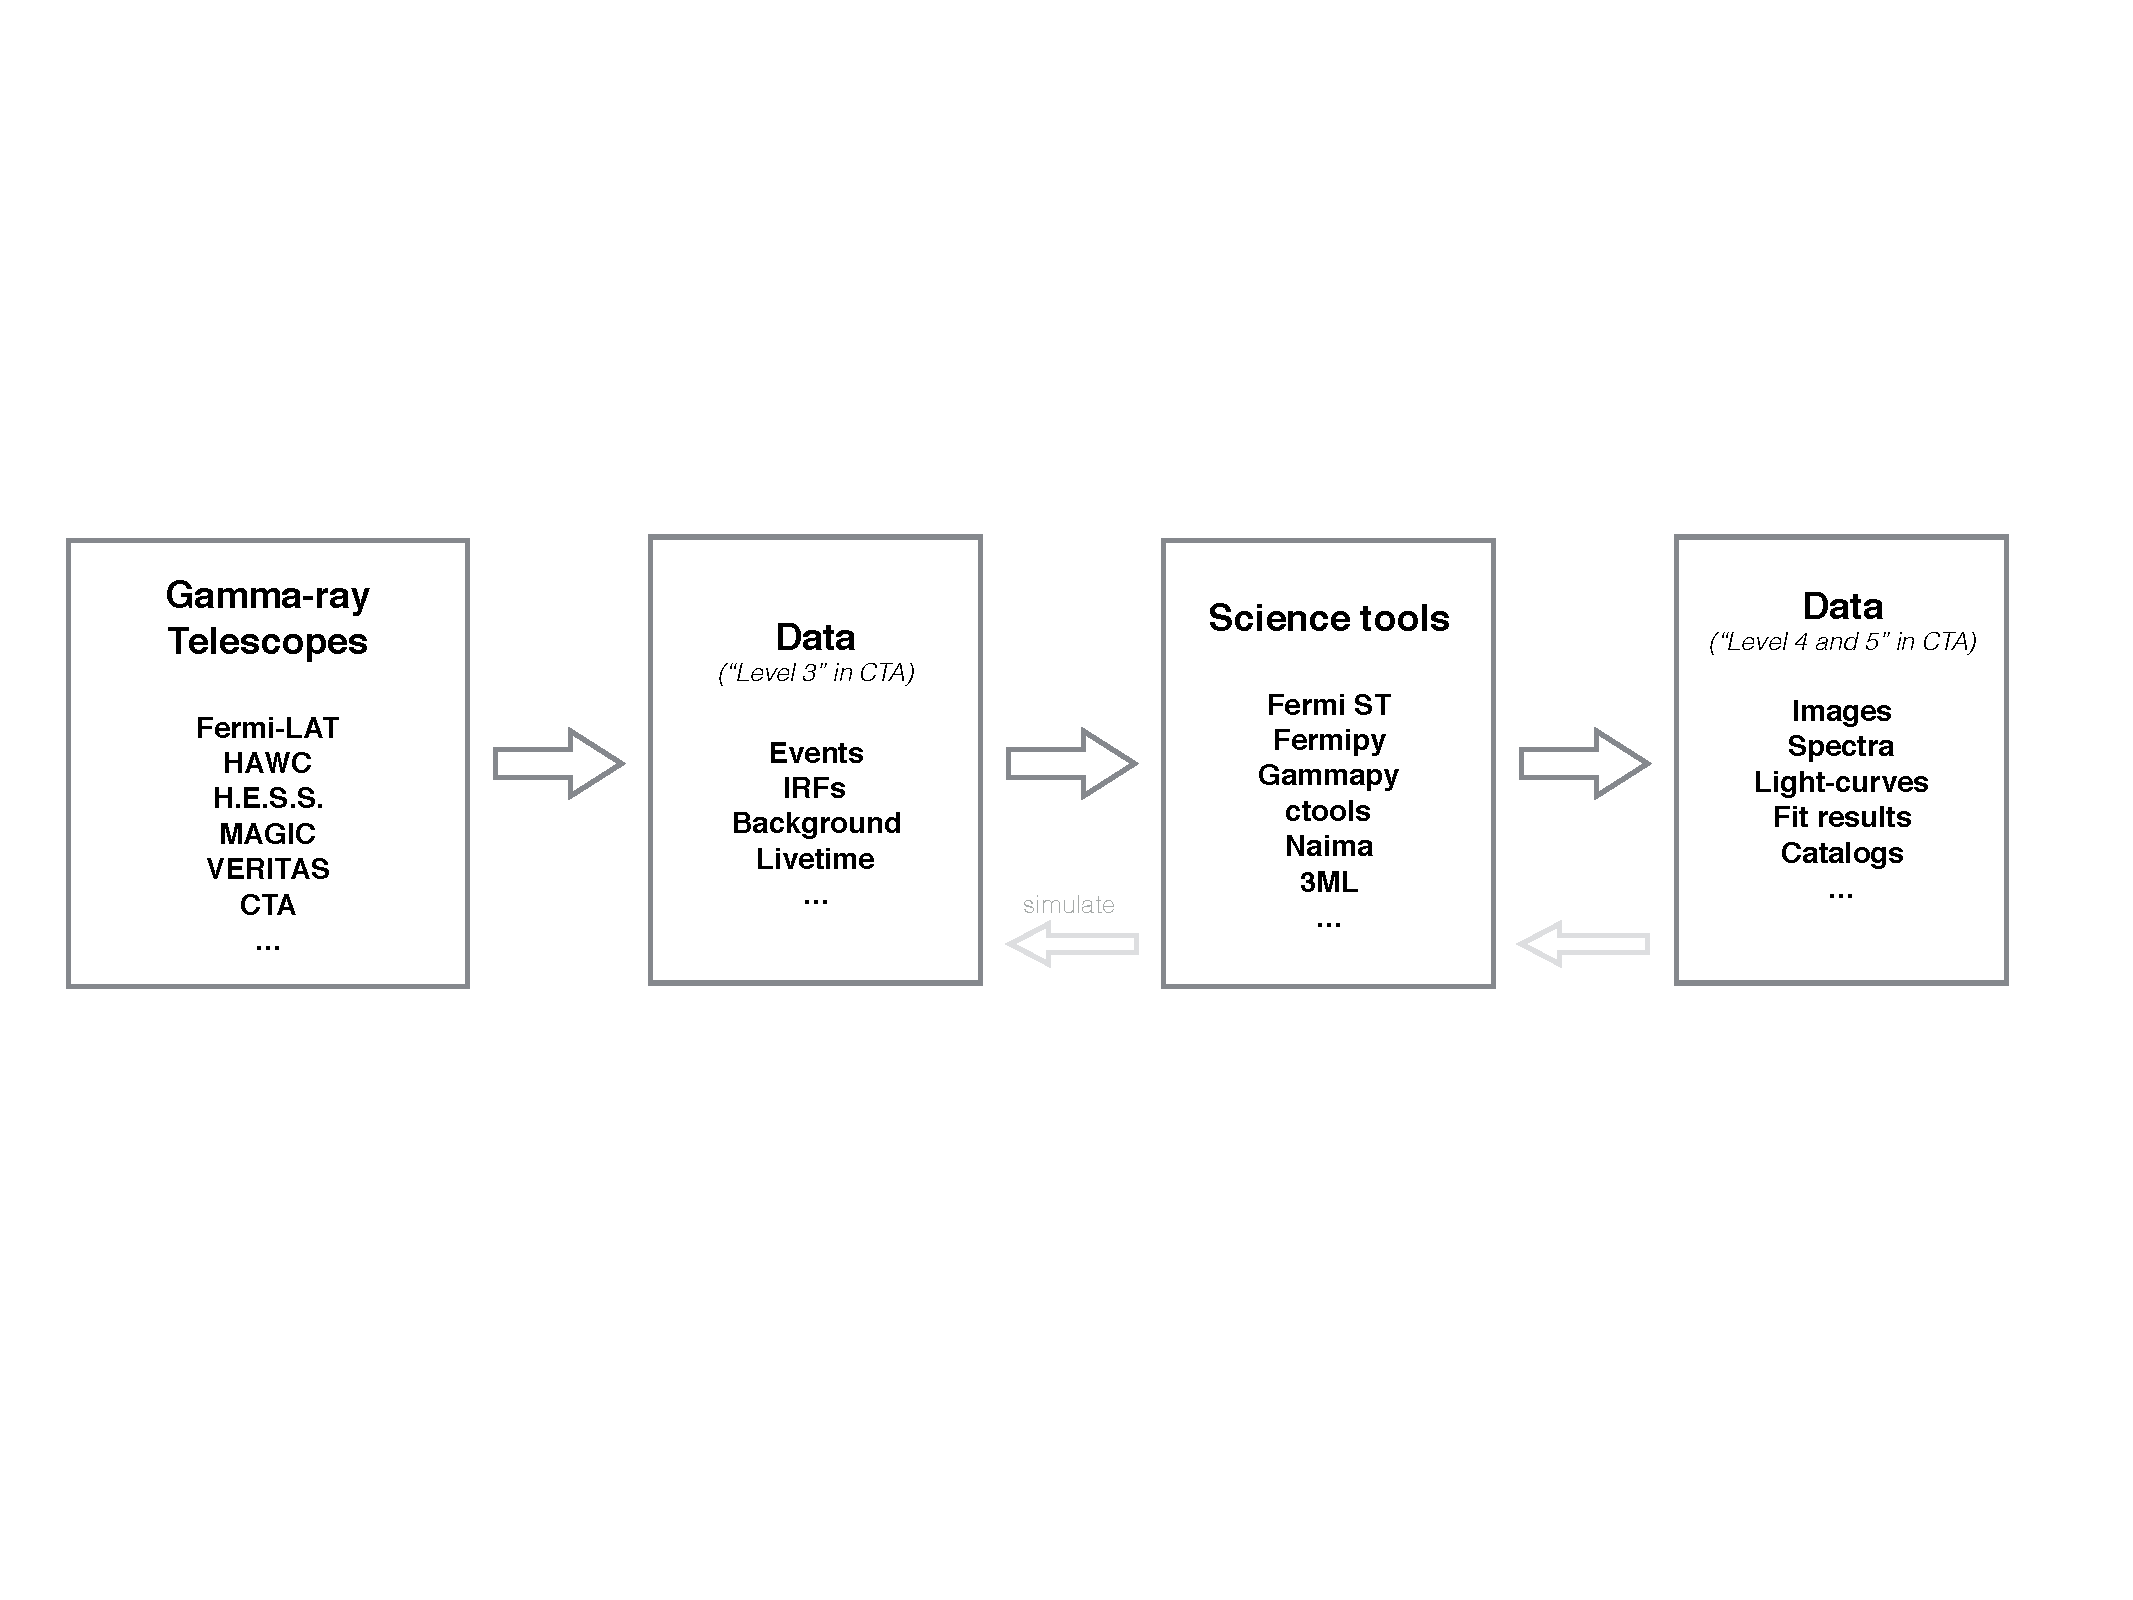
\includegraphics[width=\textwidth]{figures/purpose}}
\caption{
The purpose of the \texttt{gamma-astro-data-formats} effort is to encourage communication between high-level gamma-ray data producers, science tool developers and data analysts. The goal is to develop a common data model and format, 
to avoid duplication of efforts and confusion by astronomers working with multi-mission gamma-ray data or try alternative analysis tools.
}
\label{fig:purpose}
\end{figure}

Open source analysis tools for very-high-energy (VHE) gamma-ray astronomy have emerged. They all meet on the common ground of using FITS files for data transfer. The current generation of IACTs (H.E.S.S., MAGIC and VERITAS) all use their own private software based on the ROOT library, which prevents the analysis of the respective data with any other tool than the corresponding software. Current open source analysis tools provide alternative techniques as compared to the ones present in the VHE astronomy field. These techniques (e.g. 3D likelihood analysis such as the one already implemented for Fermi-LAT) improve the sensitivity of IACTs by roughly a 20\%. In addition, the data model of CTA is currently being developed. One of the main points of defining the high level data format for CTA is to understand the instrument including its systematic uncertainties and Instrument Response Functions (IRF)\footnote{The IRF relates the source emitted photons with the detected events, allowing the computation of gamma-ray fluxes as a function of time, energy and direction.} dependencies. Taking into account that CTA will operate as an open observatory, the needs from a user perspective have to be also taken into account to create a solution as simple as possible. Having agreed on a common data format and data store and access (folder structure), makes mid-level (event energies, positions) and high-level (source position, morphology, spectrum) data comparison between different analysis chains, algorithms and open-source tools possible. This will also ease interoperability between other codes (e.g. checking and combining results). Currently two open-source science tools packages are being developed for current IACTs and CTA data analysis, Gammapy (\cite{2015arXiv150907408D}) and ctools (\cite{2016AnA...593A...1K}). Gammapy is an in-development Astropy-affiliated package. ctools is based on the GammaLib analysis framework, which is mainly written in C++.

%TODO: also mention other codes: pointlike \citep{2010PhDT.......147K},
%Naima \citep{2015arXiv150903319Z}, 3ML \citep{2015arXiv150708343V},
%Fermipy\footnote{\fermipy}, Fermi ScienceTools.

%TODO: Is there anything we can cite for CTA data challenge 1 or data challenge 2 plans?
%TODO: Mention website and some info on how CTA is releasing IRF files at the moment (prod2)?
